\documentclass{beamer}
\usepackage[utf8]{inputenc}
\usepackage{multicol}	
\usepackage[czech]{babel}
\usepackage{animate}

\usetheme{Boadilla}
 
\graphicspath{{./Images/}}
 
\title[Prezentace BP]
{Jednoduchá hra s procedurálně generovaným obsahem}
\author{Serhiy Kudryashov}
\institute[UPOL]{Vedoucí práce: Mgr. Petr Osička, Ph.D. \linebreak
\includegraphics[width=3cm]{UP_logo_stred_cz.png}}
\date{2017}

\AtBeginSection[]
{
  \begin{frame}
    \frametitle{Obsah}
    \begin{multicols}{1}
  		\tableofcontents[currentsection,hideothersubsections]
	\end{multicols}
  \end{frame}
}

\begin{document}
 
\frame{\titlepage}

\begin{frame}{Obsah}
	\begin{multicols}{1}
  		\tableofcontents
	\end{multicols}
\end{frame}

\section{Úvod}

\begin{frame}
	\frametitle{Úvod}
	{\large Motivace:
	\begin{itemize}
		 \item Nové zkušenosti
		 \item Dozvědět více
	 	 \item Kreativní přístup
	\end{itemize}
	}
\end{frame}

\begin{frame}
	\frametitle{Úvod}
	
   {\large Dosažené cíle práce:
 
	\begin{itemize}
 		\item<2-> Prozkoumál jsem možnosti procedurálního generování obsahu v počítačových hrách
		\item<3-> Vytvořil jsem hru a na její příkladu jsem zjištěné metody implementoval
 		\item<4-> Okomentoval jsem vhodnost zjištěných metod
	\end{itemize}
	}
\end{frame}

\section{Použité technologie}
	\subsection{Unity3D}
	
\begin{frame}

	\frametitle{Unity3D}
	\begin{center}
		
\includegraphics[height=3cm]{unity-logo.jpg}	
	\end{center}
	Unity3D je herní engine vyvinutý společností Unity Technologies pro vývoj her pro PC, konzole, mobily a web. 

\end{frame}

\begin{frame}
	\frametitle{Unity3D}
	
	Možnosti Unity: 
	\begin{itemize}
 		\item 2D a 3D hry libovolného žánru
		\item {\settoheight{\dimen0}{C}C\kern-.05em \resizebox{!}{\dimen0}{\raisebox{\depth}{\bf \#}}} a Javascript
 		\item Intuitivní UI
 		\item Multiplatformní
 		\item Libovolné IDE
	\end{itemize}

\end{frame}
	
	\subsection{Adobe Photoshop}
	
\begin{frame}
	\begin{center}
		
\includegraphics[height=3cm]{photoshop-logo.png}	
	\end{center}
	\frametitle{Adobe Photoshop}
	Adobe Photoshop je bitmapový grafický editor pro tvorbu a úpravy bitmapové grafiky vytvořený firmou Adobe Systems.
\end{frame}

\section{O hře}
	\subsection{Žanr}
	\subsection{Koncept}
		
\begin{frame}
	\frametitle{Žanr a Koncept}
	Zvolení žanru a konceptu:
	\begin{itemize}
 		\item Podpora procedurálního generování
		\item Jednoduchost
 		\item Intuitivnost
	\end{itemize}
	\pause
	Výsledek: 2D Roguelike Dungeon Crawler
	\begin{center}
		
\includegraphics[height=3cm]{game-concept.png}	
	\end{center}
\end{frame}

	\subsection{Grafická stránka}
	
\begin{frame}
	\frametitle{Grafická stránka}	
	
	\begin{minipage}{0.45\linewidth}
		\begin{figure}
			\animategraphics[loop,controls,width=\linewidth]{3}{player-anim-}{0}{3}
    		\caption{Příklad animace}		
		\end{figure}    	
	\end{minipage}\hfil
	\begin{minipage}{0.55\linewidth}
	Pixel art \\Druh počítačové grafiky:
	\begin{itemize}
 		\item Vytvářen po jednotlivých pixelech(obrazových bodech)
		\item Extrémně malé obrázky (většinou)
 		\item Každý pixel musí být přesně nabarven
 		\item Každý snímek je kreslen zvlášť
	\end{itemize}
	\end{minipage}
\end{frame}


\section{Uživatelské rozhraní}
	\subsection{Hlavní menu}	
	\subsection{Ve hře}	
	
\begin{frame}
	\frametitle{Uživatelské rozhraní}
	
	\begin{multicols}{4}
  		\begin{itemize}
 			\item Počet zdraví
			\item Minimapa
 			\item Action bar
 			\item Inventář
		\end{itemize}
	\end{multicols}
	
	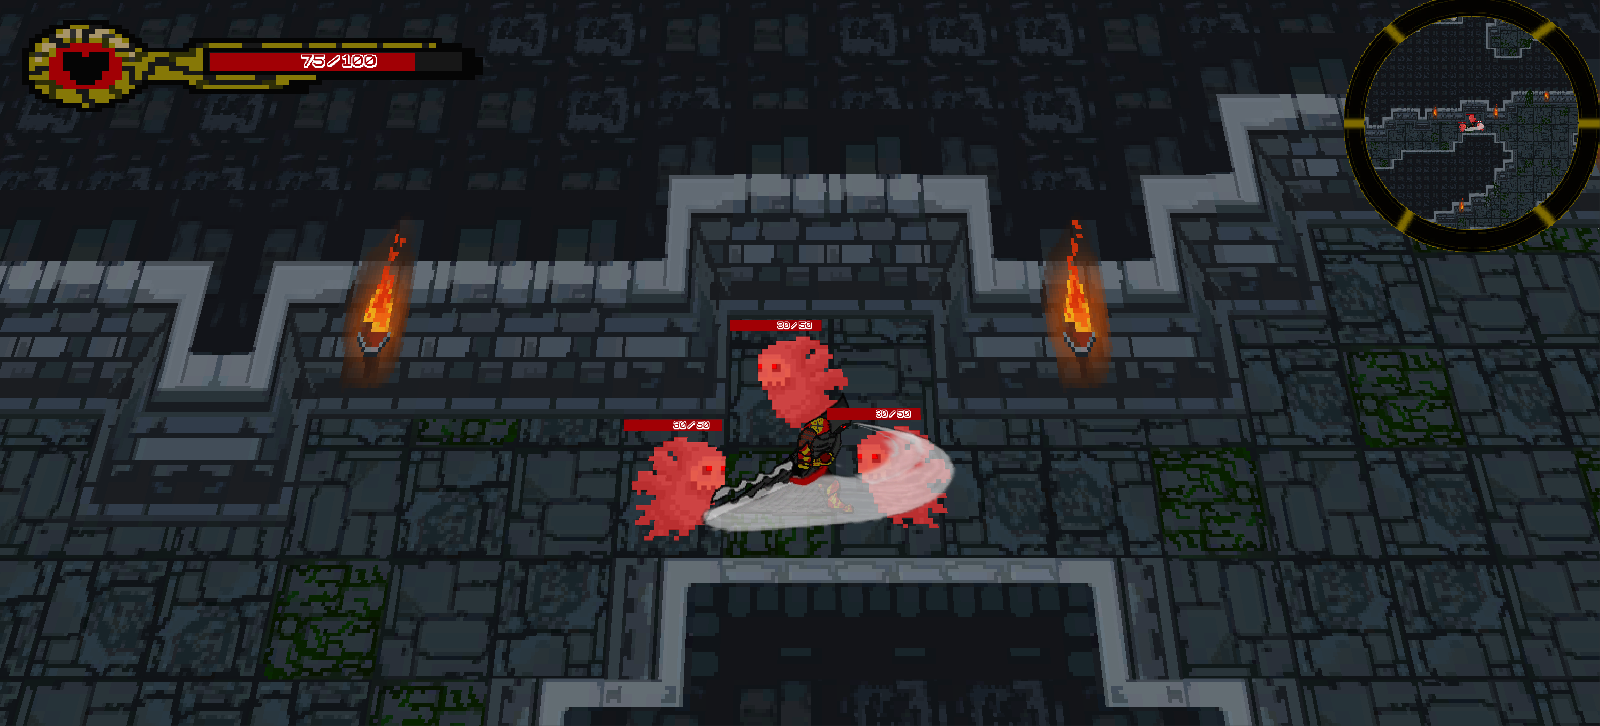
\includegraphics[width=12.3cm, height = 6.5cm]{UI-game.png}	
		
\end{frame}


\section{Procedurální generovaní}

\subsection{Výhody}
\subsection{Nevýhody}
	
\begin{frame}
\frametitle{Procedurální generovaní}
Procedurální generování se vztahuje na herní obsah, který je vytvářen algoritmicky, nikoli ručně.
	\begin{multicols}{2}
		Výhody:
  		\begin{itemize}
  			\item Nepředvídatelnost
 			\item Zrychlení vývoje
		\end{itemize}
		Nevýhody:
		\begin{itemize}
 			\item Nezaručuje nelineárnost
 			\item Nepřirozenost
		\end{itemize}
	\end{multicols}		
\end{frame}	

\begin{frame}	
	\frametitle{Procedurální generovaní}
	Procedurální generování obsahu neznamená náhodné generování obsahu.	
	\begin{multicols}{2}
		Procedurálně generovaný obsah:
  		\begin{itemize}
 			\item Vygenerované elementy
			\item Algoritmus 
		\end{itemize}
		Náhodně generovaný obsah:
		\begin{itemize}
 			\item Predefinované elementy
 			\item Sada pravidel
		\end{itemize}
	\end{multicols}		
\end{frame}
	
	\subsection{Zvolené algoritmy}
\begin{frame}
	\frametitle{Zvolené algoritmy}
	\begin{multicols}{3}
  		\begin{itemize}
 			\item Celulární automat 
			\item Perlinův šum
 			\item Voroného diagram
		\end{itemize}
	\end{multicols}
	\begin{multicols}{3}
  		
\includegraphics[width=4cm, height=4cm]{celular-ex.png}
  		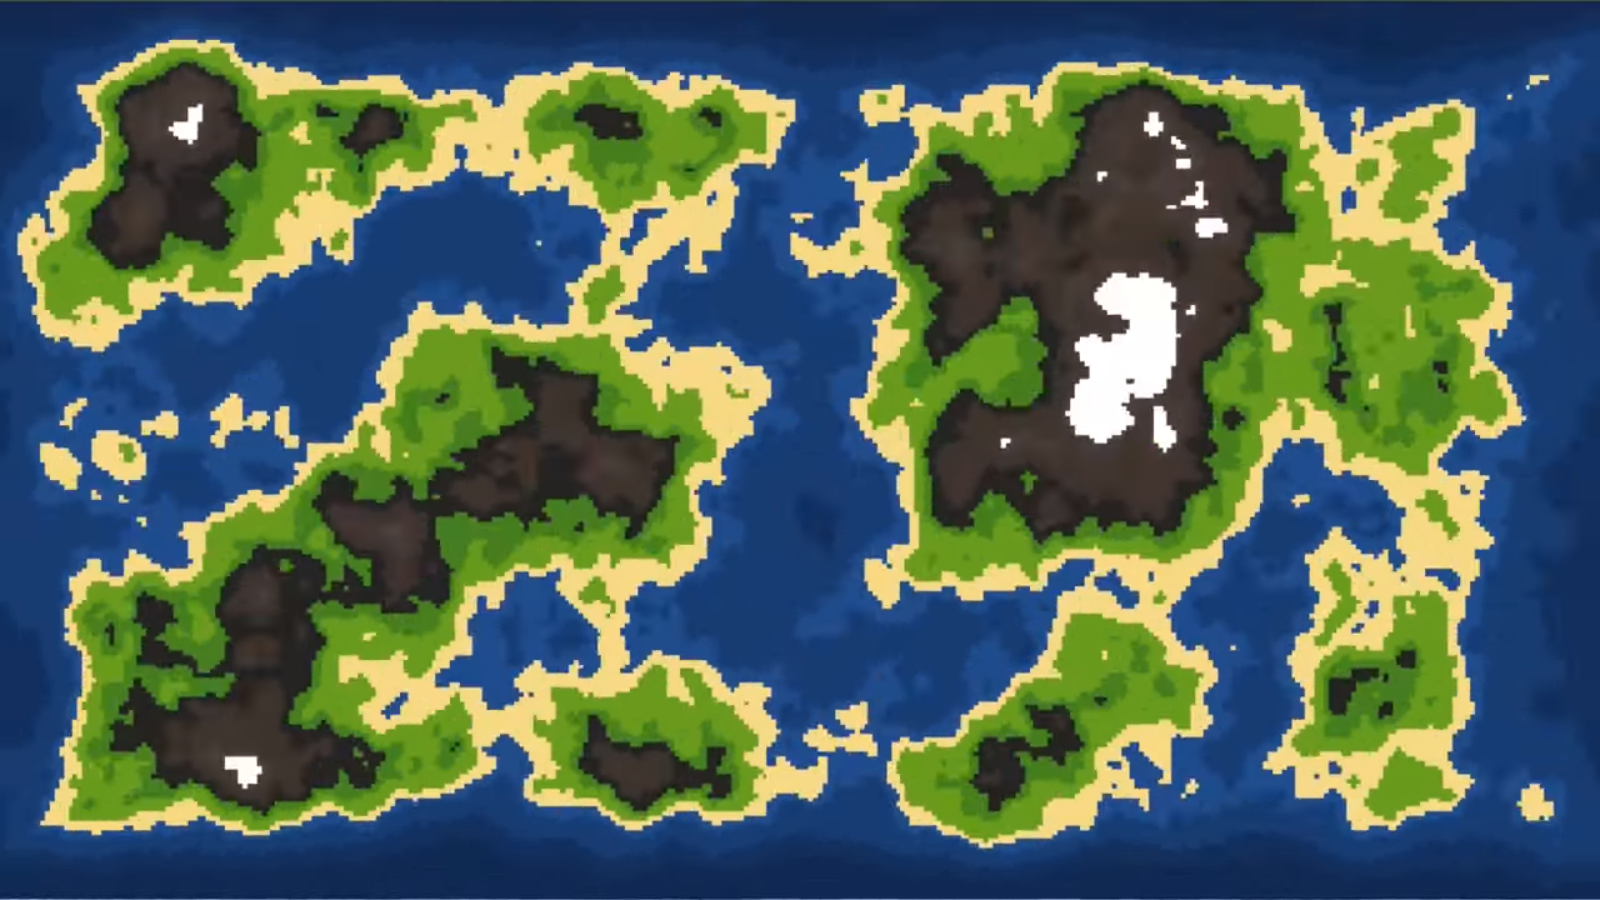
\includegraphics[width=4cm, height=4cm]{perlin-ex.png}
  		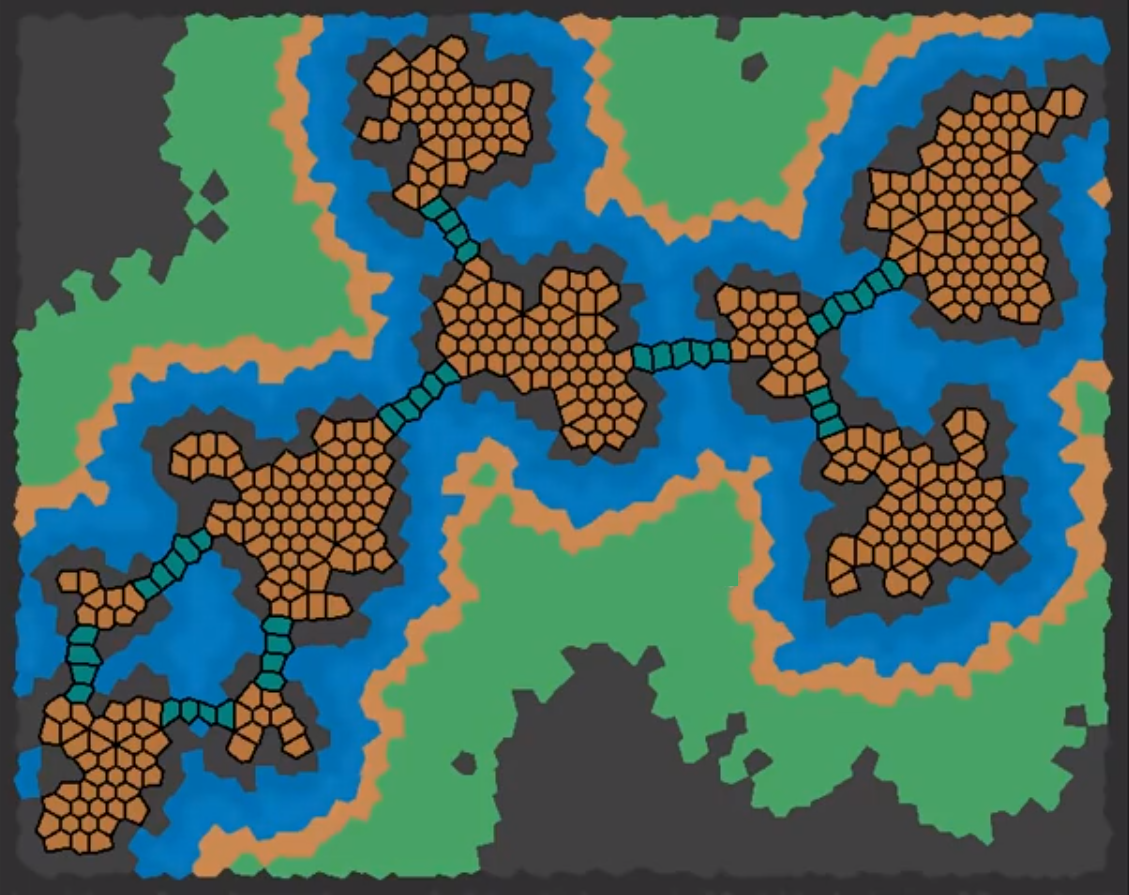
\includegraphics[width=4cm, height=4cm]{voronoi-ex.png}
	\end{multicols}
\end{frame}
	\subsection{Implementace}
	
\begin{frame}
	\frametitle{Celulární automat}
	\begin{itemize}
		\item Zaplnění mapy
		\begin{center}		
			
\includegraphics[width=\linewidth]{celular-ex2.png}	
		\end{center}	
	\end{itemize}
\end{frame}
\begin{frame}
	\frametitle{Celulární automat}
	\begin{itemize}
		\item Seskupení
		\begin{center}
			\item
			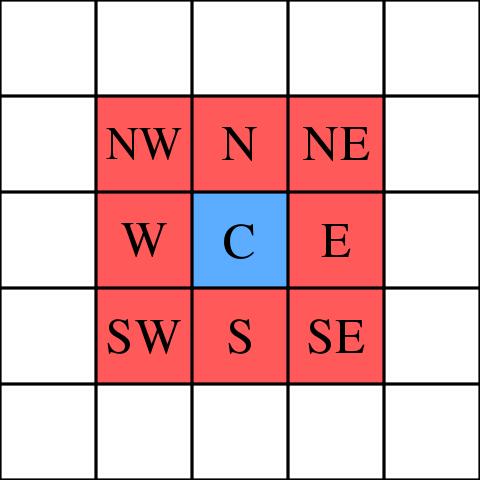
\includegraphics[width=7cm]{moore-n.png}	
		\end{center}
	\end{itemize}	
\end{frame}
\begin{frame}
	\frametitle{Celulární automat}
	\begin{itemize}
		\item Seskupení a vytvářetí průchodu
		\begin{center}
			\item
			
\includegraphics[width=\linewidth]{celular-ex3.png}	
		\end{center}
	\end{itemize}	
\end{frame}
\begin{frame}
	\frametitle{Celulární automat}
	\begin{itemize}
		\item Použití
		\begin{center}
			\item
			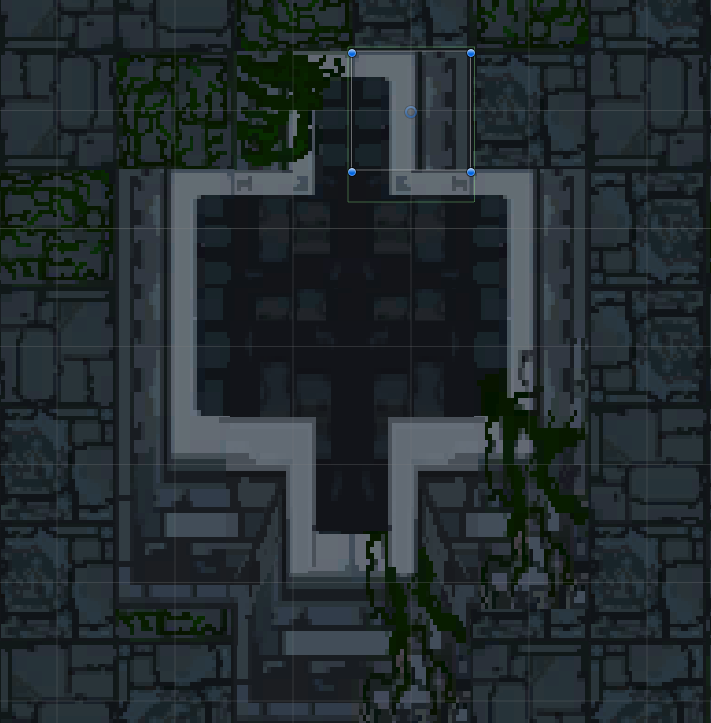
\includegraphics[width=7cm]{cave-paint.png}	
		\end{center}
	\end{itemize}	
\end{frame}
\begin{frame}
	\frametitle{Celulární automat}
	\begin{itemize}
		\item Výsledek
		\begin{center}
			\item
			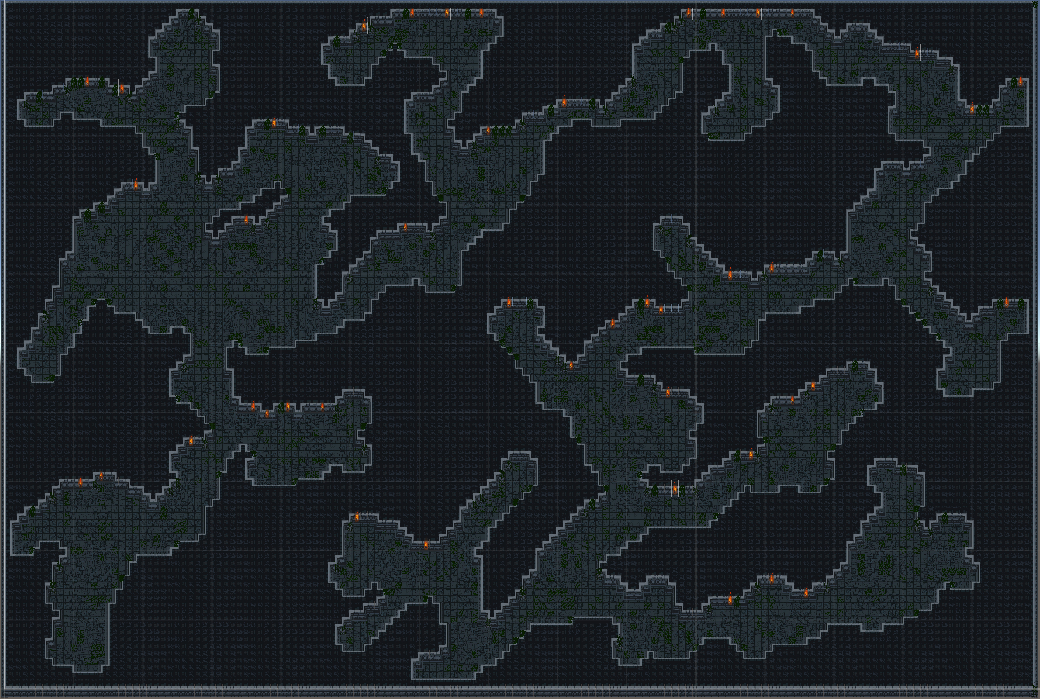
\includegraphics[width=10cm]{cave-result.png}	
		\end{center}
	\end{itemize}	
\end{frame}
\section{Závěr}
 
\end{document}